\chapter{BroodwarBotQ: putting it all together}
%%% There's no difference between a pessimist who says, "Oh it's hopeless, so don’t bother doing anything." and an optimist who says, "Don't bother doing anything, it's going to turn out fine anyways. Either way, nothing happens.
%%% --Yvon Chouinard

\begin{quotation}
\textit{Dealing with failure is easy: Work hard to improve. Success is also easy to handled: You've solved the wrong problem. Work hard to improve.}\\
\begin{flushright}Alan J. Perlis (1982)\end{flushright}
\end{quotation}

\lettrine{I}{n} this chapter, we present some of the engineering that went in the robotic player's (bot) implementation. We will also present the different flows of informations and how decisions are made during a game. Finally we will present the results of the full robotic player to various bots competitions.

\chaptertoc

\begin{figure}
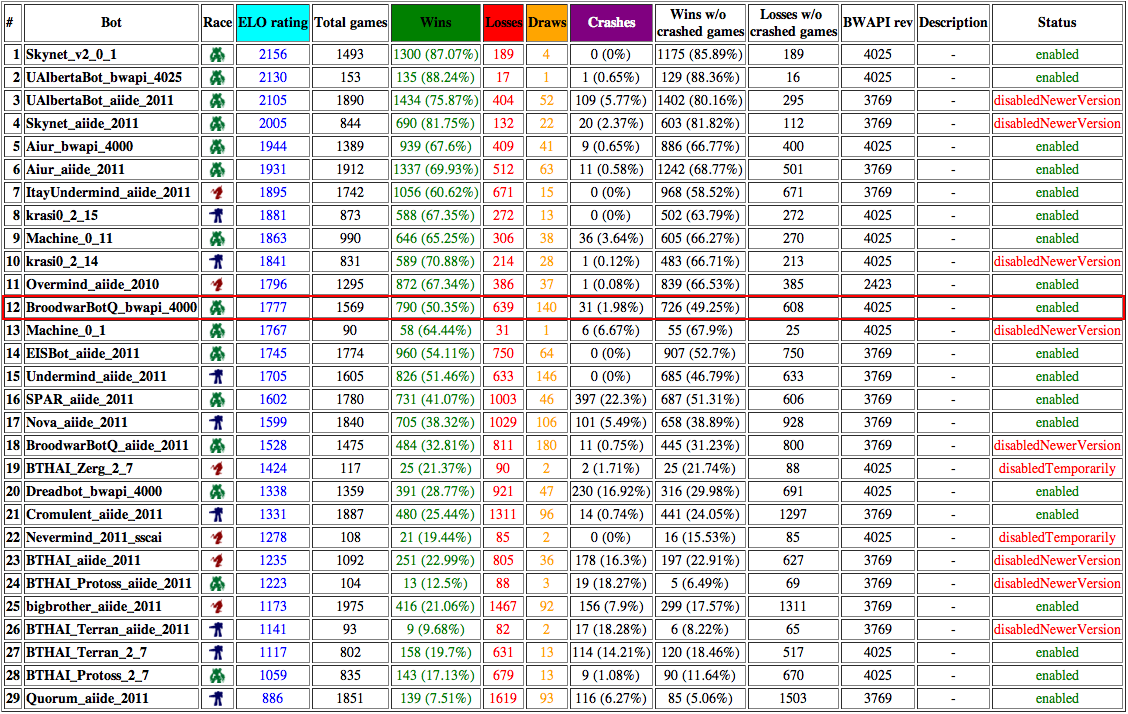
\includegraphics[width=1.0\columnwidth]{images/ladder_2012-02-12.png}
\caption{Bots ladder on February 12th, 2012. With \textsc{BroodwarBotQ} using a Bayesian model for opponent's strategy prediction as well as for \glos{micro}.}
\end{figure}


\section{Code Architecture}
mapping schéma code <-> schéma info-flow.


\section{A Game Walkthrough}
The tree of decisions.


\section{Results}
AIIDE 2010,2011, Ladder.


